\newpage

\subsubsection{UCA 5 - Monitoraggio dello storico degli accessi dell'utente}
\begin{figure}[h]
	\centering	
	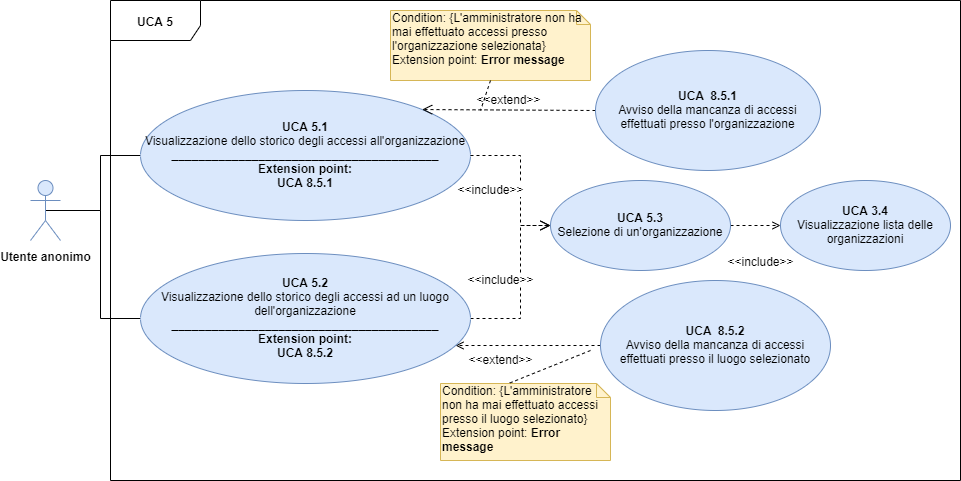
\includegraphics[scale=0.5]{sezioni/UseCase/Immagini/UCA5.png}
	\caption{UCA 5 - Monitoraggio dello storico degli accessi dell'utente}
\end{figure}

\begin{itemize}
    \item \textbf{Attori primari:} Utente anonimo, Utente riconosciuto
    \item \textbf{Precondizione:} L'utente ha precedentemente scaricato la lista delle organizzazioni.
    \item \textbf{Postcondizione:} L'ha visualizzato lo storico degli accessi relativo all'organizzazione desiderata oppure al luogo desiderato dell'organizzazione scelta.
    \item \textbf{Scenario principale:} L'utente selezionerà l'organizzazione desiderata dalla lista delle organizzazioni e quindi la funzionalità per mostrare lo storico degli accessi oppure un luogo specifico per analizzarne il relativo storico degli accessi.
\end{itemize}

\subsubsection{UCA 5.1 - Visualizzazione dello storico degli accessi all'organizzazione}
\begin{itemize}
    \item \textbf{Attori primari:} Utente anonimo, Utente riconosciuto
    \item \textbf{Precondizione:} L'utente ha precedentemente scaricato la lista delle organizzazioni.
    \item \textbf{Postcondizione:} L'utente ha visualizzato lo storico degli accessi (con nome dell'organizzazione, timestamp di ingresso, di uscita, e tempo di permanenza) presso l'organizzazione scelta. Se si trova all'interno dell'organizzazione stessa, viene visualizzato il tempo passato al suo interno dall'ultimo ingresso effettuato.
    \item \textbf{Scenario principale:} L'utente esegue la procedura per visualizzare lo storico degli accessi effettuati presso l'organizzazione desiderata.
    \item \textbf{Scenario alternativo:} L'utente non è mai entrato nell'organizzazione selezionata, pertanto verrà visualizzato un avviso informativo [UCA 7.5.1].
    \item \textbf{Flusso di eventi:}
    \begin{enumerate}
        \item L'utente seleziona l'organizzazione interessata [UCA 5];
        \item L'utente seleziona la funzionalità per mostrare gli accessi effettuati presso l'organizzazione selezionata;
        \item L'utente ha la possibilità di ordinare gli accessi all'organizzazione [UCA 5.1.1] [UCA 5.1.2] oppure di effettuare una ricerca tra di essi per gli accessi di uno specifico giorno [UCA 5.1.3].
    \end{enumerate}
    \item \textbf{Inclusioni:}
    \begin{itemize}
        \item UCA 5 - Selezione di un'organizzazione;
    \end{itemize}
    \begin{itemize}
        \item UCA 7.5.1 - Avviso della mancanza di accessi effettuati presso l'organizzazione selezionata.
    \end{itemize}
\end{itemize}

\subsubsection{UCA 5.2 - Visualizzazione dello storico degli accessi ad un luogo dell'organizzazione}
\begin{itemize}
    \item \textbf{Attori primari:} Utente anonimo, Utente riconosciuto
    \item \textbf{Precondizione:} L'utente sta visualizzando lo storico accessi di un'organizzazione [UCA 5] e l'organizzazione in questione deve avere almeno un luogo registrato.
    \item \textbf{Postcondizione:} L'utente visualizza lo storico degli accessi (con nome del luogo, timestamp di ingresso, di uscita, e tempo di permanenza) al luogo desiderato. Se l'utente dovesse trovarsi all'interno del luogo stesso, viene visualizzato il tempo passato al suo interno dall'ultimo ingresso effettuato.
    \item \textbf{Scenario principale:} L'utente esegue la procedura per visualizzare lo storico degli accessi effettuati presso il luogo desiderato.
    \item \textbf{Scenario alternativo:} L'utente non è mai entrato nel luogo selezionato, pertanto verrà mostrato un avviso informativo [UCA 7.5.2].
    \item \textbf{Flusso di eventi:}
    \begin{enumerate}
        \item L'utente seleziona l'organizzazione interessata [UCA 5];
        \item L'utente seleziona un luogo tra quelli offerti dall'organizzazione selezioanta;
        \item L'utente seleziona la funzionalità per mostrare gli accessi effettuati presso il luogo selezionato;
        \item L'utente ha la possibilità di ordinare gli accessi al luogo [UCA 5.2.1] [UCA 5.2.2] oppure di effettuare una ricerca tra di essi per gli accessi di uno specifico giorno [UCA 5.2.3].
    \end{enumerate}
    \item \textbf{Estensioni:}
    \begin{itemize}
        \item UCA 7.5.2 - Avviso della mancanza di accessi effettuati presso il luogo selezionato.
    \end{itemize}
\end{itemize}

\subsubsection{UCA 5.1.1 - Ordinamento per data decrescente della lista degli accessi presso un'organizzazione}
\begin{itemize}
    \item \textbf{Attori primari:} Utente anonimo, Utente riconosciuto
    \item \textbf{Precondizione:} L'utente sta visualizzando lo storico accessi di un'organizzazione [UCA 5].
    \item \textbf{Flusso di eventi:}
    \begin{enumerate}
        \item L'utente seleziona la funzionalità per riordinare lo storico di accessi dell'organizzazione per data in ordine decrescente.
    \end{enumerate}
    \item \textbf{Postcondizione:} L'utente ottiene la lista di accessi iniziale riordinata per data in ordine decrescente.
\end{itemize}

\subsubsection{UCA 5.1.2 - Ordinamento per data crescente della lista degli accessi presso un'organizzazione}
\begin{itemize}
    \item \textbf{Attori primari:} Utente anonimo, Utente riconosciuto
    \item \textbf{Precondizione:} L'utente sta visualizzando lo storico accessi di un'organizzazione [UCA 5].
    \item \textbf{Flusso di eventi:}
    \begin{enumerate}
        \item L'utente seleziona la funzionalità per riordinare lo storico di accessi dell'organizzazione per data in ordine crescente.
    \end{enumerate}
    \item \textbf{Postcondizione:} L'utente ottiene la lista di accessi iniziale riordinata per data in ordine crescente.
\end{itemize}

\subsubsection{UCA 5.1.3 - Ricerca degli accessi presso un'organizzazione in un giorno specifico}
\begin{itemize}
    \item \textbf{Attori primari:} Utente anonimo, Utente riconosciuto
    \item \textbf{Precondizione:} L'utente sta visualizzando lo storico accessi di un'organizzazione [UCA 5].
    \item \textbf{Flusso di eventi:}
    \begin{enumerate}
        \item L'utente seleziona la funzionalità per visualizzare solo gli acessi avvenuti in un giorno specifico presso l'organizzazione;
        \item L'utente seleziona il giorno desiderato.
    \end{enumerate}
    \item \textbf{Postcondizione:} L'utente ottiene la lista di accessi effettuati nel giorno selezionato.
\end{itemize}

\subsubsection{UCA 5.2.1 - Ordinamento per data decrescente della lista degli accessi presso un luogo di un'organizzazione}
\begin{itemize}
    \item \textbf{Attori primari:} Utente anonimo, Utente riconosciuto
    \item \textbf{Precondizione:} L'utente sta visualizzando lo storico accessi di un luogo [UCA 5.1].
    \item \textbf{Flusso di eventi:}
    \begin{enumerate}
        \item L'utente seleziona la funzionalità per riordinare lo storico di accessi del luogo per data in ordine decrescente.
    \end{enumerate}
    \item \textbf{Postcondizione:} L'utente ottiene la lista di accessi iniziale riordinata per data in ordine decrescente.
\end{itemize}

\subsubsection{UCA 5.2.2 - Ordinamento per data crescente della lista degli accessi presso un luogo di un'organizzazione}
\begin{itemize}
    \item \textbf{Attori primari:} Utente anonimo, Utente riconosciuto
    \item \textbf{Precondizione:} L'utente sta visualizzando lo storico accessi di un luogo [UCA 5.1].
    \item \textbf{Flusso di eventi:}
    \begin{enumerate}
        \item L'utente seleziona la funzionalità per riordinare lo storico di accessi del luogo per data in ordine crescente.
    \end{enumerate}
    \item \textbf{Postcondizione:} L'utente ottiene la lista di accessi iniziale riordinata per data in ordine crescente.
\end{itemize}

\subsubsection{UCA 5.2.3 - Ricerca degli accessi presso un luogo di un'organizzazione in un giorno specifico}
\begin{itemize}
    \item \textbf{Attori primari:} Utente anonimo, Utente riconosciuto
    \item \textbf{Precondizione:} L'utente sta visualizzando lo storico accessi di un luogo [UCA 5.1].
    \item \textbf{Flusso di eventi:}
    \begin{enumerate}
        \item L'utente seleziona la funzionalità per visualizzare solo gli acessi avvenuti in un giorno specifico presso il luogo in questione dell'organizzazione;
        \item L'utente seleziona il giorno desiderato.
    \end{enumerate}
    \item \textbf{Postcondizione:} L'utente ottiene la lista di accessi effettuati presso il luogo in questione nel giorno selezionato.
\end{itemize}

\subsubsection{UCA 5.3 - Selezione di un'organizzazione}
\begin{figure}[h]
	\centering	
	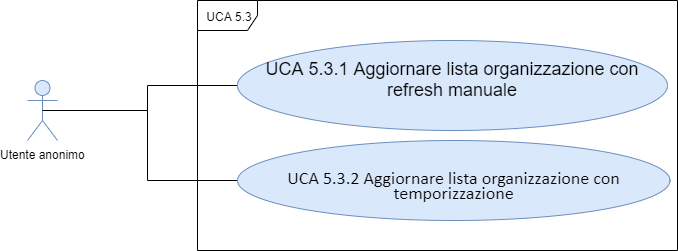
\includegraphics[scale=0.5]{sezioni/UseCase/Immagini/UCA5.3.png}
	\caption{UCA 5.3 - Selezione di un'organizzazione}
\end{figure}

\begin{itemize}
    \item \textbf{Attori primari:} Utente anonimo, Utente riconosciuto
    \item \textbf{Precondizione:} L'utente ha precedentemente scaricato la lista delle organizzazioni.
    \item \textbf{Postcondizione:} L'utente ha selezionato un'organizzazione dalla lista.
    \item \textbf{Scenario principale:} L'utente selezionerà l'organizzazione desiderata dalla lista delle organizzazioni.
    \item \textbf{Flusso di eventi:}
    \begin{enumerate}
        \item L'utente visualizza la lista delle organizzazioni [UCA 3.4];
        \item L'utente seleziona dalla lista l'organizzazione interessata.
    \end{enumerate}
    \item \textbf{Inclusioni:}
    \begin{itemize}
        \item UCA 3.4 - Visualizzazione lista delle organizzazioni;
    \end{itemize}
\end{itemize}